\begin{pastexam}[label={px:ntu-109-ee-ds-21}]{臺大電機所 109 學年度（B）第 21 題}
（複選；每題 4 分，每答錯一個選項倒扣 0.8 分至該題 0 分止）

In this exam: The height of a singleton tree is defined as 0.

Consider the red-black tree in Fig.2
\begin{enumerate}[label=(\Alph*)]
\item In Fig.2, after top-down inserting the key 86, then the color of key 86 is red.
\item In Fig.2, after top-down inserting the key 9, then the parent of key 9 is key 13.
\item In Fig.2, after top-down deleting the key 87, then the color of key 85 is red.
\item In Fig.2, after top-down deleting the key 10, then the parent of key 13 is key 15.
\item The 2-3-4 tree representation of Fig.2 has height 2.
\end{enumerate}

\begin{center}
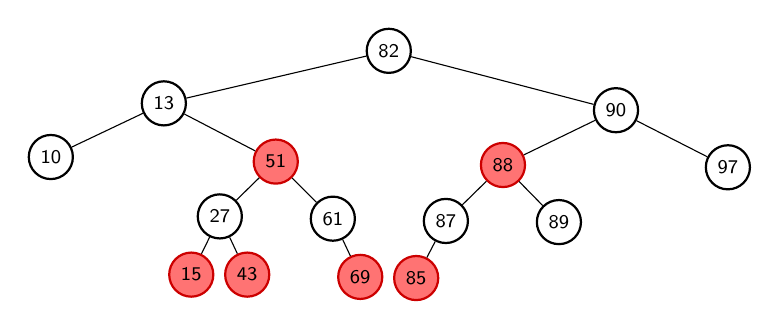
\begin{tikzpicture}[x=1.45cm,y=1.45cm,v/.style={draw,thick,circle,minimum size=5.6mm,inner sep=0pt,font=\scriptsize\sffamily},
  r/.style={v,draw=red!80!black,fill=red!55}]
  \foreach \n/\x/\y in {82/7.13/6.68,13/5.16/7.14,90/9.12/7.20,10/4.17/7.61,97/10.10/7.70,27/5.65/8.13,61/6.64/8.15,87/7.63/8.17,89/8.62/8.18} {
    \node[v] (\n) at (\x,-\y) {\n};
  }
  \foreach \n/\x/\y in {51/6.14/7.65,88/8.13/7.68,15/5.40/8.64,43/5.89/8.64,69/6.88/8.66,85/7.37/8.67} {
    \node[r] (\n) at (\x,-\y) {\n};
  }
  \foreach \a/\b in {82/13,82/90,13/10,13/51,51/27,51/61,27/15,27/43,61/69,90/88,90/97,88/87,88/89,87/85} { \draw (\a) -- (\b); }
\end{tikzpicture}\\ Fig.2 Red-black tree
\end{center}
\end{pastexam}

\begin{pastsoln}
答案：(E)。 （(D) 和刪除時「兩種旋轉都可以用」的選擇有關，見下面的說明；本書採用的規則下 (D) 錯。）

Fig.2 中紅色的節點是 $51, 88, 15, 43, 69, 85$，其他是黑色。 檢查：每條從根到外部節點的路徑上都有
$3$ 個黑節點（例如 $82, 13, 10$；$82, 13, 27$；$82, 90, 87$），沒有相鄰的紅節點，是合法的紅黑樹。

「由上而下」（top-down）的插入和刪除是 Weiss 課本的做法：從根往下走一趟，邊走邊調整，走到底就
完成，不用再往回走。 資結書第~10.3~節講的是由下而上的做法，第~11.1.5~節講 2-3-4 樹由上而下的插入，
紅黑樹的由上而下插入就是它的翻版。 每個選項都從 Fig.2 原本的樹開始做。

\textbf{由上而下插入的規則。} 從根往下找插入位置，經過的節點 $X$ 如果兩個子節點都是紅的，就做顏色
翻轉（$X$ 變紅、兩個子節點變黑，相當於把 2-3-4 樹的 4-節點先分裂）；翻轉後如果 $X$ 和它的父節點都
是紅的，像由下而上那樣做單旋轉或雙旋轉。 走到底把新鍵當成紅色的葉節點接上，父節點是紅的就再旋轉
一次。 最後根塗黑。

\textbf{(A) 插入 86：錯。} 路徑 $82 \to 90 \to 88 \to 87 \to 85$，途中沒有節點的兩個子節點都是紅的
（$90$ 的子節點 $88$ 紅、$97$ 黑；$87$ 只有一個紅色子節點），不用翻轉。 $86 > 85$，接在 $85$ 的右邊，
是紅的。 父節點 $85$ 也是紅的，祖父 $87$ 是黑的：$85$ 是 $87$ 的左子節點，$86$ 是 $85$ 的右子節點，
是之字形（LR），做雙旋轉，$86$ 升上來並塗黑，$85$、$87$ 塗紅：
\begin{center}
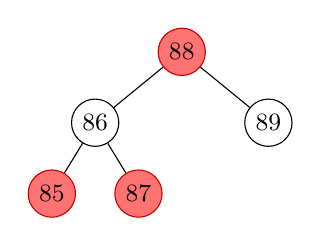
\begin{tikzpicture}[level distance=9mm,every node/.style={circle,draw,minimum size=6mm,inner sep=0pt,font=\small},
  r/.style={draw=red!80!black,fill=red!55},
  level 1/.style={sibling distance=22mm},level 2/.style={sibling distance=11mm}]
\node[r] {88} child {node {86} child {node[r] {85}} child {node[r] {87}}} child {node {89}};
\end{tikzpicture}
\end{center}
$86$ 是黑色。

\textbf{(B) 插入 9：錯。} 路徑 $82 \to 13 \to 10$，途中沒有節點的兩個子節點都是紅的（$13$ 的子節點 $10$
黑、$51$ 紅）。 $9 < 10$，接在 $10$ 的左邊，紅色；父節點 $10$ 是黑的，不用調整。 $9$ 的父節點是 $10$。

\textbf{由上而下刪除的規則。} 刪除最後都歸結成刪除一片葉子：有兩個子節點，或只有右子節點的節點，用
右子樹最小的鍵取代，改刪那個節點；只有左子節點的，用左子樹最大的鍵取代。 刪紅色的葉子很簡單，
所以往下走的時候要設法讓「目前節點」$X$ 變成紅的。 令 $P$ 是 $X$ 的父節點、$T$ 是 $X$ 的兄弟。 開始時
把根當成 $X$，它的父節點（虛擬的）當成紅的。 每到一個新的 $X$，都保持 $P$ 紅、$X$ 和 $T$ 黑：
\begin{enumerate}
\item $X$ 的兩個子節點都是黑的（外部節點算黑）：
\begin{enumerate}
\item $T$ 的兩個子節點也都是黑的：顏色翻轉，$P$ 變黑、$X$ 和 $T$ 變紅。
\item $T$ 的外側子節點（離 $X$ 較遠的那個）是紅的：對 $P$、$T$ 做單旋轉，$T$ 升上來塗紅，$P$ 和那個
外側子節點塗黑，$X$ 塗紅。
\item 否則 $T$ 的內側子節點是紅的：雙旋轉，那個內側子節點升上來塗紅，$P$、$T$ 塗黑，$X$ 塗紅。
\end{enumerate}
\item $X$ 有一個紅色子節點：直接往下走一層。 新的 $X$ 如果是紅的就繼續往下；如果是黑的，它的兄弟
$T$ 一定是紅的，把 $T$ 和 $P$ 旋轉（$T$ 塗黑、$P$ 塗紅），回到情形 1。
\end{enumerate}
$T$ 的兩個子節點\textbf{都是紅的}時，1(b) 和 1(c) 都合法，結果不同。 本書照課本列出的順序，先看外側
子節點，所以這時用 1(b) 的單旋轉（和資結書第~10.3.7~節由下而上刪除的情況 4「遠側子節點 $f$ 是紅的就單旋轉，
不管近側的顏色」一致）。

\textbf{(C) 刪除 87：錯。} $87$ 只有左子節點 $85$，改成用 $85$ 取代 $87$，再刪掉原本 $85$ 那片葉子。
往下走：$X = 82$，兩個子節點 $13$、$90$ 都黑，情形 1(a)，$82$ 暫時變紅。 $X = 90$（黑），子節點 $88$ 是
紅的，情形 2，往下走到 $88$，紅的，繼續。 $X = 87$（黑），有紅色子節點 $85$，情形 2，往下走到 $85$，
紅的。 $85$ 是紅色的葉子，直接刪掉，$85$ 這個鍵搬到原本 $87$ 的節點，那個節點是黑的。 最後根 $82$
塗回黑色。 結果 $88$ 的子節點是 $85$（黑）和 $89$（黑），$85$ 是黑色。

\textbf{(D) 刪除 10：錯（採用本書的規則）。} 往下走：
\begin{itemize}
\item $X = 82$：子節點 $13$、$90$ 都黑，情形 1(a)，$82$ 暫時變紅。
\item $X = 13$（黑），$P = 82$（紅），$T = 90$（黑）。 $13$ 有紅色子節點 $51$，情形 2，往下走到 $10$。
\item $X = 10$ 是黑的，兄弟 $T = 51$ 是紅的：把 $51$ 和 $13$ 旋轉，$51$ 升上來塗黑，$13$ 塗紅。 現在
$P = 13$（紅），$X = 10$，$T = 27$（黑）。
\item $X = 10$ 的兩個子節點都是外部節點（黑）。 $T = 27$ 的兩個子節點 $15$、$43$ 都是紅的；外側
（離 $10$ 較遠）的是 $43$，用 1(b)：對 $13$、$27$ 單旋轉，$27$ 升上來塗紅，$13$ 和 $43$ 塗黑，$10$
塗紅。 $15$ 原本是 $27$ 的左子節點，旋轉後接到 $13$ 的右邊。
\item $10$ 是紅色的葉子，刪掉。 根 $82$ 塗回黑色。
\end{itemize}
結果左半邊：
\begin{center}
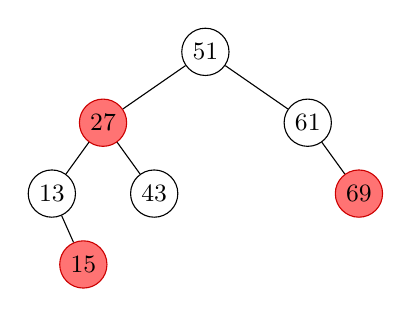
\begin{tikzpicture}[level distance=9mm,every node/.style={circle,draw,minimum size=6mm,inner sep=0pt,font=\small},
  r/.style={draw=red!80!black,fill=red!55},
  level 1/.style={sibling distance=26mm},level 2/.style={sibling distance=13mm},level 3/.style={sibling distance=8mm}]
\node {51} child {node[r] {27} child {node {13} child[missing] child {node[r] {15}}} child {node {43}}}
  child {node {61} child[missing] child {node[r] {69}}};
\end{tikzpicture}
\end{center}
$13$ 的父節點是 $27$。 每條路徑仍有 $3$ 個黑節點（例如 $82, 51, 13$；$82, 51, 43$）。 如果在 $15$、$43$
都紅時改用 1(c) 的雙旋轉，$15$ 會升上來成為 $13$ 和 $27$ 的父節點，刪掉 $10$ 後 $13$ 的父節點就是
$15$，(D) 變成對的。 本題的答案取決於這個選擇；照課本先列外側的順序，(D) 錯。

\textbf{(E) 對。} 紅黑樹對應 2-3-4 樹：每個黑節點和它的紅色子節點合成一個 2-3-4 樹的節點（資結書
第~11.1.6~節）。 Fig.2 對應：根 $\{82\}$；第二層 $\{13, 51\}$、$\{88, 90\}$；第三層 $\{10\}$、
$\{15, 27, 43\}$、$\{61, 69\}$、$\{85, 87\}$、$\{89\}$、$\{97\}$。 共三層，依本題的定義（只有根時高度
$0$）高度是 $2$。 一般來說，2-3-4 樹的層數就是紅黑樹每條根到外部節點路徑上的黑節點數（這裡是 $3$），
高度是 $3 - 1 = 2$。
\end{pastsoln}
